\documentclass[12pt]{article}
%\usepackage[margin=1in]{geometry}
\usepackage[left=1.2cm, right=1.2cm, top=2cm]{geometry}
\usepackage{amsmath, amsthm, amssymb, amsfonts}
\usepackage{scrextend}
\usepackage{graphicx}
\usepackage{multicol}


% Set up stuff to handle Python code nicely.
\usepackage{listings}
\usepackage{color}

\definecolor{codegreen}{rgb}{0,0.6,0}
\definecolor{codegray}{rgb}{0.5,0.5,0.5}
\definecolor{codepurple}{rgb}{0.58,0,0.82}
\definecolor{backcolour}{rgb}{0.95,0.95,0.92}

\lstdefinestyle{mystyle}{
    backgroundcolor=\color{backcolour},
    commentstyle=\color{codegreen},
    keywordstyle=\color{magenta},
    numberstyle=\tiny\color{codegray},
    stringstyle=\color{codepurple},
    basicstyle=\footnotesize,
    breakatwhitespace=false,
    breaklines=true,
    captionpos=b,
    keepspaces=true,
    numbers=left,
    numbersep=5pt,
    showspaces=false,
    showstringspaces=false,
    showtabs=false,
    tabsize=2
}

\lstset{style=mystyle}

\setlength{\columnsep}{0.3in}

\newcommand{\N}{\mathbb{N}}
\newcommand{\Z}{\mathbb{Z}}

\newenvironment{problem}[2][Problem]{\begin{trivlist}
\item[\hskip \labelsep {\bfseries #1}\hskip \labelsep {\bfseries #2.}]}{\end{trivlist}}
%If you want to title your bold things something different just make another thing exactly like this but replace "problem" with the name of the thing you want, like theorem or lemma or whatever

\newenvironment{answer}[2][Answer]{\begin{trivlist}
\item[\hskip \labelsep {\bfseries #1}\hskip \labelsep {\bfseries #2.}]}{\end{trivlist}}

% Enable one-column figures in multicol.
\newenvironment{Figure}
  {\par\medskip\noindent\minipage{\linewidth}}
  {\endminipage\par\medskip}

\newcommand\textlcsc[1]{\textsc{\MakeLowercase{#1}}}

\begin{document}

%\renewcommand{\qedsymbol}{\filledbox}
%Good resources for looking up how to do stuff:
%Binary operators: http://www.access2science.com/latex/Binary.html
%General help: http://en.wikibooks.org/wiki/LaTeX/Mathematics
%Or just google stuff

% \title{AST 221: Problem Set 1}
% \author{Jonas Powell}
% \maketitle


%make title bold and 14 pt font (Latex default is non-bold, 16 pt)
\title{\Large \textbf{Galactic Astronomy: Problem Set 1}}

\author{
{\rm Jonas Powell, \textit{Wesleyan University}}\\
}


\maketitle


\begin{addmargin}[4em]{4em}
\noindent {\bf Due: Thursday, Feb. 7 by midnight.} Late papers are not accepted. If you cannot complete the assignment, hand in what you have completed before the deadline. Consider the deadline to be like the boarding time for an airplane, or the deadline for a grant submission to NASA or NSF. If you miss the deadline, you do not get on the airplane, no matter how good your excuse is. If you miss an NSF or NASA deadline, you do not get the grant, no matter how good your project is. The best advice is ... finish early. You can submit multiple times, right up to the deadline. Whatever your latest submission is, when the deadline occurs, is what will be graded.
\bigskip \bigskip
\end{addmargin}

 
% \textbf{
% TO DO: \\
% - Check all values with someone \\
% - Clean up code (maybe make scratch file and official file? Maybe not. \\
% - Prettier header?)\\
% - Check the velocities in P4
% }


% Begin two-column layout
\begin{multicols*}{2}


\begin{problem}{1} Convert the commonly used speed unit of km s$^{-1}$ into a useful unit system for galactic astronomy, pc My$^{-1}$. That is, 1 kilometer per second equals how many parsecs per million years?

\end{problem}

\begin{answer}{1}
  For this problem, we could pretty easily just Google the answer, but it's more fun to work it out unit by unit instead. We begin with the distances. \bigskip

  We would like to convert parsecs to km. We know that there are 206,265 AU/PC, and that 1 AU = 150 million km. Therefore,

  \begin{align*}
    1 \text{ parsec} = 206265 \times 1.5 \times 10^8 \text{ km}
  \end{align*}

  For the time component, we recall that 1 My = 10$^{6}$ years, and that a year is made up of 60 seconds/minute, 60 minutes/hour, 24 hours/day, and 365 days/year (more or less). The product of this series is 31,536,000 seconds/year. Therefore, the time component is given by
  % 31536000 = 3.1536e7
  \begin{align*}
    1 \text{ My} &= 10^{6} \times (3.1536 \times 10^7) \\
                 &= 3.1536 \times 10^{13} \text{ seconds}
  \end{align*}

  Putting it all together, we find:
  \begin{align*}
    1 \text{ pc My$^{-1}$} &= \frac{206265 \times 1.5 \times 10^8 \text{ km}}{3.1536 \times 10^{13} \text{ seconds}} \\
      &\approx 0.98 \text{ km s$^{-1}$} \\
    \rightarrow 1 \text{ km s$^{-1}$} &= 1.02 \text{ pc My$^{-1}$}
  \end{align*}
  % \rightarrow 1 \text{ seconds My$^{-1}$}} &= 1.02 \text{pc My$^{-1}$}

  This is pretty wild! It's saying that a My and parsec have almost exactly the same relationship as the kilometer and second. That's neat. \bigskip

  A note on uncertainties: I am assuming that a year is made up of nice round, consistent number of hours/minutes/seconds, neglecting the reality of leap years/seconds/etc. However, I feel alright doing this because an My is so much bigger than the scale of those fluctuations that any errors in our astronomical velocity measurement are likely far more consequential than these errors. \bigskip
\end{answer}




\bigskip \bigskip
\begin{problem}{2} Calculate the value of the constant in the equation:
$$v_t = \text{const} \mu d$$
where v$_t$ has the units km s$^{-1}$, $\mu$ is in arc-seconds y$^{-1}$ and d is in pc.
\end{problem}

\begin{answer}{2}

% [km/s] = k * [arcsec/year] * [pc]
% k = [km year]/[arcsec pc = AU] = [year * (km/AU = 150 million] = 150 million years
To solve this, we may represent each variable by its units, letting $k$ represent our constant, and solve.

\begin{align*}
  \text{[km/s]} &= k \times \text{[arcsec/year]} \times \text{[pc]} \\
  k &= \text{[km year]}/\text{[s arcsec pc]} \\
    &= [\frac{\text{year}}{\text{s}}] [\frac{\text{km}}{\text{arcsec pc = AU}}] \\
    &= (3.17 \times 10^{-8}) (1.5 \times 10^8) \\
    &= 4.755 \\
\end{align*}

We find a final value for our conversion constant of $k = 4.755$.

\end{answer}






\bigskip \bigskip
\begin{problem}{3} Write a computer program that transforms a given RA, Dec (J2000) to galactic coordinates (l,b). Test your program against a Web site that does the same transformation. Be sure to test it for both positive and negative declinations. [Hint: Make sure it works in the tricky region between 0 degrees and -1 degrees�.,, such as  RA = 04:37:48, Dec = -0:21:25. Also be sure it gives the right answer near the galactic center, l=0.]

\end{problem}

\begin{answer}{3}
Please find the relevant code attached at the end of this file in the function \texttt{radec\_to\_galactic()}. Testing done on the given example, Vega, and a couple others showed functionality.
\end{answer}





\bigskip \bigskip
\begin{problem}{4} A fictional G2V star has the following known properties:

Position = 04:24:46.0, +12:37:22.0 (J2000)

Parallax (p) = 0.025$''$

Proper motion  = -5.0 mas yr$^{-1}$ (RA), +24.0 mas yr$^{-1}$ (Dec)

Heliocentric radial velocity (v$_r$) = +28.0 km/s

\bigskip

\noindent Determine the following information for this star. Use appropriate units for galactic astronomy.

Galactic Coordinates (l,b)

Distance (d)

Magnitude of the proper motion vector ($\mu$)

Position Angle of the proper motion vector (PA)

Transverse velocity (v$_t$)

Speed relative to the Sun (v$_{space}$)

What constellation is this star in?

Is it closer to or further from the center of the Galaxy than the Sun?

\end{problem}

\begin{answer}{4}


Relevant values are given in the table below. Please find my calculations for these values in the Star class in the code attached at the end of this problem set.

\bigskip
\begin{Figure}
  \centering
  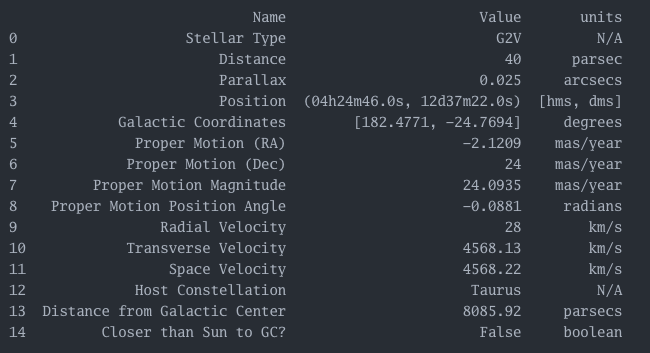
\includegraphics[width=\linewidth]{prob4.png}
  % \caption{Given and calculated values for the hypothetical star provided. Formulae used for these calculations are given in the Star class definition in the code at the end of this problem set.}
  % \label{fig:prob4}
\end{Figure}
\bigskip

\end{answer}







\begin{problem}{5} The Gaia Mission is able to measure positional accuracy in the best cases to about 10 $\mu$as (micro arc-seconds)!

a) Give an example of what 10 $\mu$as is in terms of everyday experience, i.e. something you could a general audience with, to explain to them how good this instrument is at resolving angles.

b) Given its ability to detect proper motions of about 10 $\mu$as y$^{-1}$ would Gaia be capable of observing grass growing on the Moon, (assuming grass could grow on the Moon)? If not, from what distance could it observe grass growing? (Be sure to state your assumptions.)

c) Could Gaia detect the rotation of the Andromeda galaxy? (Again, be sure to state any assumptions you make.)

d) Is Gaia capable of detecting the proper motion of a typical quasar? (.... assumptions...)

\end{problem}

\begin{answer}{5}
10 $\mu$as is a really small number - $10 \times 10^{-6} [\frac{\text{as}}{\mu\text{as}}] \times 206265^{-1} [\frac{\text{radians}}{\text{as}}] \approx 5 \times 10^{-11}$ radians. To get a feel for what that means, we can use the small angle approximation for tangent and say $\tan{\theta} \approx \theta = 5 \times 10^{-11} =$ O/A, so let's think about finding something that is eleven orders of magnitude - again, \textlcsc{eleven orders of magnitude} - smaller than something else.

\bigskip
\noindent \textbf{Part A: }Let's say our smaller object is 1mm in scale; in this case, we should be looking for a length that is of order $10^8$ meters, or hundreds of thousands of kilometers (to reclaim that coefficient of 5 that was in our conversion, let's say we are looking at length scales of around 500,000 km). \bigskip

Let's first identify a potential source. A quick Google search of $''$millimeter sized things$''$ informed me that, while a penny is a little too big (it's tens of millimeters across), it seems that, in the "United States of America" lettering at the top of the non-Abe Lincoln side of the penny, each letter looks to be of order 1.5x1mm. \bigskip

Now that we have our source object, let's figure out how far away Gaia could be while still resolving that source. Conveniently enough (leading into the next part of this question), the moon is a little under 400,000 km away from Earth. While that isn't \textit{quite} far enough to actually stretch our resolution to its limit, it still is pretty darn far. \bigskip

Now we can put that all together into one sentence: If Gaia were on Earth\footnote{...and if it was callibrated to be able to focus on the Moon, and if there didn't exist line-of-sight issues like atmosphere, etc etc.}, and if Neil Armstrong had accidentially dropped a penny, face down, when he hopped out onto the Moon, we could resolve the lettering in $''$United States of America$''$ on that little tiny piece of copper. That's pretty spectacular. \bigskip

\textlcsc{ADDENDUM:} It has come to my attention that a lot of people in the class chose the penny-on-the-moon example. While I now wish I had been a little more original, I'm still so blown away by the scenario that I'm just keeping it anyways, originality be damned.

\bigskip
\noindent \textbf{Part B: } According to TheGrassPeople.com\footnote{ https://thegrasspeople.com/how-long-grass-grow}, grass grows at a pace of around 2-3 cm/week (this feels like too large a number, but since these are order-of-magnitude calculations, it's fine), which we'll call 1 cm/week $\rightarrow$ 50 cm/year. This number is well above our detection limit of $5 \times 10^{-11}$ radians year$^{-1} \approx 1 \text{ mm year}^{-1}$.

\bigskip
\noindent \textbf{Part C: } According to the first plot of Andromeda's rotation curve that I plucked from Google Images\footnote{ https://ned.ipac.caltech.edu/level5/Sept16/Bertone/Figures/figure3.jpg}, Andromeda rotates at around 200 km/s (obviously with radial variations, but let's ignore those for now) and is around 2.5 million light years away. We may convert this to km/year by multiplying by $3 \times 10^{7}$, the approximate number of seconds in a year, yielding $6 \times 10^{9}$ km/year.

At its distance of around 2.5 million light years $\approx 2.4 \times 10^{19}$ km from us, we may find that Andromeda rotates at

\begin{align*}
  \frac{v}{d} &= \frac{6 \times 10^{9}}{2.4 \times 10^{19}} \\
              &\approx 2.5 \times 10^{-10} \text{radians/year} \\
              &\approx 0.5 \, \mu \text{as year$^{-1}$} \\
\end{align*}

With an angular resolution of about 10 $\mu$as year$^{-1}$, this means that we are about an order of magnitude away from being able to actually detect the rotation of the Andromeda Galaxy.

\bigskip
\noindent \textbf{Part D: } Since quasars typically are held to be objects with no proper motion, then Gaia would of course be unable to detect any motion. There are a number of publications that discuss the fact that many of the quasars in the Gaia database do, in fact, show proper motion, but since these are atypical, they are not terribly relevant to this question.

\end{answer}


\begin{problem}{6} With the precision that the Gaia Mission reaches for many stars, a level of about 60 $\mu$as per measurement, could it detect the wobble of the Sun due to Jupiter from a distance of 10 pc, assuming it made enough observations over a sufficiently long period of time?

\end{problem}

\begin{answer}{6}
We must begin this problem by assessing how far apart the center of mass and the stellar core are in a system comprised of a Sun-mass star and a Jupiter-mass/major axis planet. Using the center-of-mass equation, we may do this relatively easily. Setting the origin of this calculation to be the star's center and drawing on known values for a Solar mass, Jovian mass, and Jupiter's semi-major axis, we find:

\begin{align*}
  x_{\text{CoM}} &= \frac{m_{\odot} x_{\odot} + m_{\text{Jup}} x_{\text{Jup}}}{m_{\odot} + m_{\text{Jup}}} \\
    &= \frac{(1.9 \times 10^{27} \text{ kg}) (7.78 \times 10^{11} \text{m})}{1.9 \times 10^{27} \text{ kg} + 2 \times 10^{30} \text{ kg}} \\
    &= 7.3 \times 10^8 \text{ meters}
\end{align*}

This means that the barycenter of this system would be a mere 70,000 km away from the star's center.

We may now find the parallax angle that would be caused by such a motion by taking the ratio of twice that distance (as it swings from side to side over the course of a year) over the 10 parsecs that we are observing from.

\begin{align*}
  p &= \frac{1.46\times 10^9 \text{ meters}}{10 \text{ parsecs} = 3\times 10^{17} \text{ meters}} \\
  &= 4.8 \times 10^{-9} \text{ radians} \\
  &= 10^{-3} \text{ arcsec}
\end{align*}

This is obviously significantly more than the 60$\mu$as per measurement, meaning that it would be relatively easy to detect the wobble of the Sun caused by Jupiter from 10pc with Gaia.



\end{answer}
\end{multicols*}
\vfill\eject
\clearpage


\lstinputlisting[language=Python]{hw1_scratch.py}





\end{document}
